\documentclass[pdf]{beamer}
\usetheme{Madrid} % You can change this to other themes like Madrid, Copenhagen, etc.
\usecolortheme{default}
\usepackage{tabularx}
\usepackage{lscape}
\usepackage{graphicx}
\usepackage{tikz}\usetikzlibrary{arrows.meta,calc} %library tikz
% Packages for math and symbols
\usepackage{amsmath, amssymb}
\usepackage{graphicx} % For including images if needed
\usepackage[utf8]{inputenc}

% Title slide information
\title{Semi-stable lattices in higher rank}


\author{Tri Nguyen}


\begin{document}

% Title Slide
\begin{frame}
    \titlepage
\end{frame}

% Outline Slide
\begin{frame}{Outline}
    \tableofcontents
\end{frame}

\section{Introduction}
\begin{frame}{Historical motivation}
    Serre [1977] and Quillen [see Grayson, 1982] used the notion of semistable vector
    bundle on an algebraic curve to study $\text{SL}_n(\mathcal{O})$ when $\mathcal{O}$ is a Dedekind domain finitely generated over a finite field. Stuhler
    then realized he can used the same method to adapt some work of Harder and Narasimhan on stable vector bundles to yields new facts
    about lattices in a Euclidean space.
\end{frame}
\begin{frame}
    Due to \cite{} , it is heuristical that the semi-stable lattices are the lattices in which the successive minima are closed.
\end{frame}
\begin{frame}{Definition of two-dimensional lattices}
    \begin{block}{Lattice}
        A lattice $L \subset \mathbb{R}^2$ is a set of the form
        \[L = \mathbb{Z}e_1\oplus\mathbb{Z}e_2\]
        where $e_1,e_2$ are linearly independent over $\mathbb{R}$.
    \end{block}
\end{frame}
\begin{frame}{Example of a lattice}
    \begin{figure}[h]
        \centering
        \resizebox{70mm}{70mm}{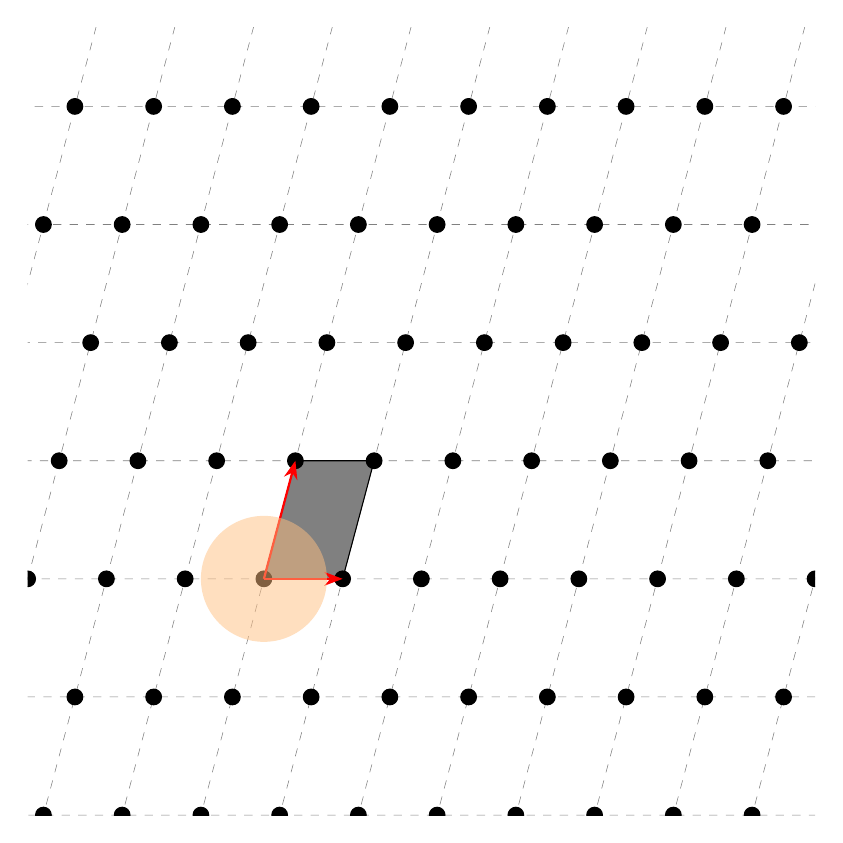
\begin{tikzpicture}
                \begin{scope}
                    \clip (0,0) rectangle (10cm,10cm); % Clips the picture...
                    \pgftransformcm{1}{0}{0.4}{1.5}{\pgfpoint{3cm}{3cm}} % Adjusted transformation matrix for less skew

                    \draw[style=help lines,dashed] (-14,-14) grid[step=1cm] (14,14); % Draws a grid in the new coordinates
                    \filldraw[fill=gray, draw=black] (0,0) rectangle (1,1); % Puts the shaded rectangle
                    \foreach \x in {-7,-6,...,7}{                           % Two indices running over each
                            \foreach \y in {-7,-6,...,7}{                       % node on the grid we have drawn 
                                    \node[draw,circle,inner sep=2pt,fill] at (\x,\y) {}; % Places a dot at those points
                                }
                        }
                    % Draw the vector from (0,0) to (1,0) in the transformed coordinate system
                    \draw[red, -Stealth, thick] (0,0) -- (1,0); % Vector from (0,0) to (1,0)
                    \draw[red, -Stealth, thick] (0,0) -- (0,1); % Vector from (0,0) to (0,1)

                \end{scope}
                % Place the circle at the lowest-left vertex (3,3) in the original coordinate system
                \fill[orange!50,semitransparent] (3,3) circle (.8cm); % Radius is 1.3cm to contain the shorter edge
            \end{tikzpicture}}
        \caption{Example of a lattice}
        \label{fig:example}
    \end{figure}
\end{frame}



\section{In 2 dimensional}
\begin{frame}{Classification of lattices}
    Do we know all the possible 2 dimensional "lattice shape"?\vspace{3em}

    \pause
    \textbf{Answer:} Up to maginifcation, rotation and change of basis, the answer is yes.
\end{frame}
\begin{frame}{Fundamental domain}
    Up to rorations and magnifications, we can reduce a lattice
    \[L = \mathbb{Z}\omega_1 \oplus \mathbb{Z}\omega_2\]
    to a lattice of the form
    \[L_z = \mathbb{Z}z\oplus\mathbb{Z}, \quad \Im(z)>0\]
    So the upper half-plane parametrizes the 2 dimensional lattices.
    \begin{block}{Classification of unit lattices}
        The map $z \mapsto \mathbb{Z}z\oplus\mathbb{Z}$ induces a bijection
        \[\text{SL}_2(\mathbb{Z}) \backslash\mathbb{H} \cong \left\lbrace \text{ lattices}\right\rbrace/\mathbb{C^\times}\]
    \end{block}

\end{frame}
\begin{frame}{Fundamental domain}
    So we reduce to study the space of lattices by looking the action of $\text{SL}_2(\mathbb{Z})$ on the upper half plane. Geometrically, the domain is given by
    \[\mathfrak{D} = \left\lbrace z=x+iy \in \mathbb{H}: |z| \ge 1,-1/2 \le x \le 1/2 \right\rbrace \],
    \pause
    \[
        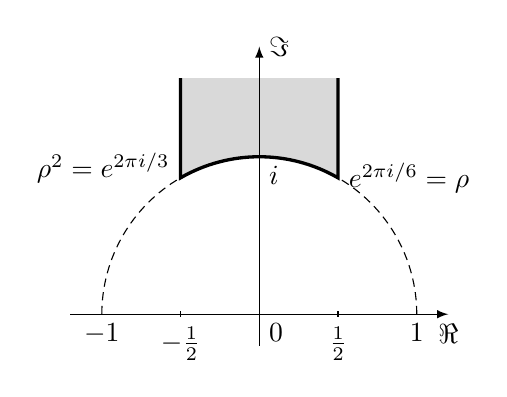
\begin{tikzpicture}[scale=2]
            \draw[densely dashed] (1,0) arc (0:60:1) (-1,0) arc (180:120:1);
            \draw[very thick, fill=gray!30] (.5,1.5) --node[right, pos=1]{$e^{2\pi i/6}=\rho$} (60:1) arc (60:120:1)
            --node[left, pos=.1]{$\rho^2=e^{2\pi i/3}$} (-.5,1.5);
            \draw[-latex] (-1.2,0) -- (1.2,0)node[below]{$\Re$};
            \draw[-latex] (0,-.2) -- (0,1.7)node[right]{$\Im$};
            \path(-1,0) --node[below, pos=0]{$-1$}node[below right, pos=.5]{0}node[below, pos=1]{1} (1,0)
            (0,1)node[below right]{$i$};
            \draw(-.5,.02)--(-.5,-.02)node[below]{$-\frac{1}{2}$}(.5,.02)--(.5,-.02)node[below]{$\frac{1}{2}$};
        \end{tikzpicture}\]
\end{frame}

\begin{frame}{Canonical plot}
    Grayson associated each lattice $L$ to some kind of \textbf{Newton polygon}. \pause

    The process is as follows:
    \begin{enumerate}
        \item Put $(0,0)$ to the plot.
        \item For each primitive vector $v \in L$, he assigns the point $(1,\log(||v||))$ to the plot.
        \item Put the point $(2,\log(vol(L)))$ to the plot.
    \end{enumerate}
\end{frame}
\begin{frame}{Canonical plot}
    \begin{figure}[h]
        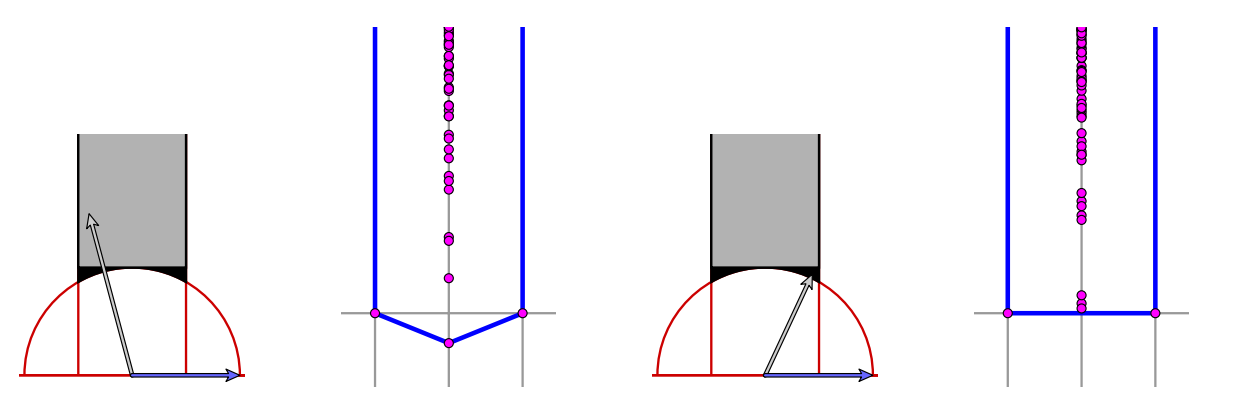
\includegraphics[width = \textwidth]{Canonical plot.png}
        \caption{The figure on the left corresponds to $z = -2/5 +3i/2$ and on the right corresponds to $z = 7/16+15i/16$}
    \end{figure}
\end{frame}
\begin{frame}{Canonical plot}
    Since the lattice is discrete, there is a shortest primitive vector - on the plot we have the lowest point.\pause\vspace{3em}

    Grayson called the set of points plotted above as \textbf{Canonical plot}. The convex hull of the collection
    of the plot point is called \textbf{profile}.
\end{frame}
\begin{frame}
    For any $z \in \mathbb{H} = \left\lbrace \text{Im}(z)>0 \right\rbrace$, we can assign to it a unit lattices
    \[z \mapsto L_z = \mathbb{Z}\dfrac{e_1}{\sqrt{y}} + \mathbb{Z}\left(\dfrac{x}{\sqrt{y}}e_1+\sqrt{y}e_2 \right)\]
    The shortest vector is then $ e_1/\sqrt{y}$, with length $\dfrac{1}{\sqrt{y}}$. So for $y<1$, the lowest
    point is below the horizontal axis.
    \pause \vspace{2em}

    The element $z$ corresponds to the lattice $L_z$ such that its lowest point on the
    vertical line $x=1$ lies below the $x$-axis is called \textbf{semi-stable}, otherwise it is called \textbf{unstable}.
\end{frame}
\begin{frame}
    Since the semi-stability is preserved under the action of $\text{SL}_2(\mathbb{Z})$, the semi-stable locus in the
    upper half plane $\mathbb{H}$ is as follows

\end{frame}
\begin{frame}
    \begin{figure}[h]
        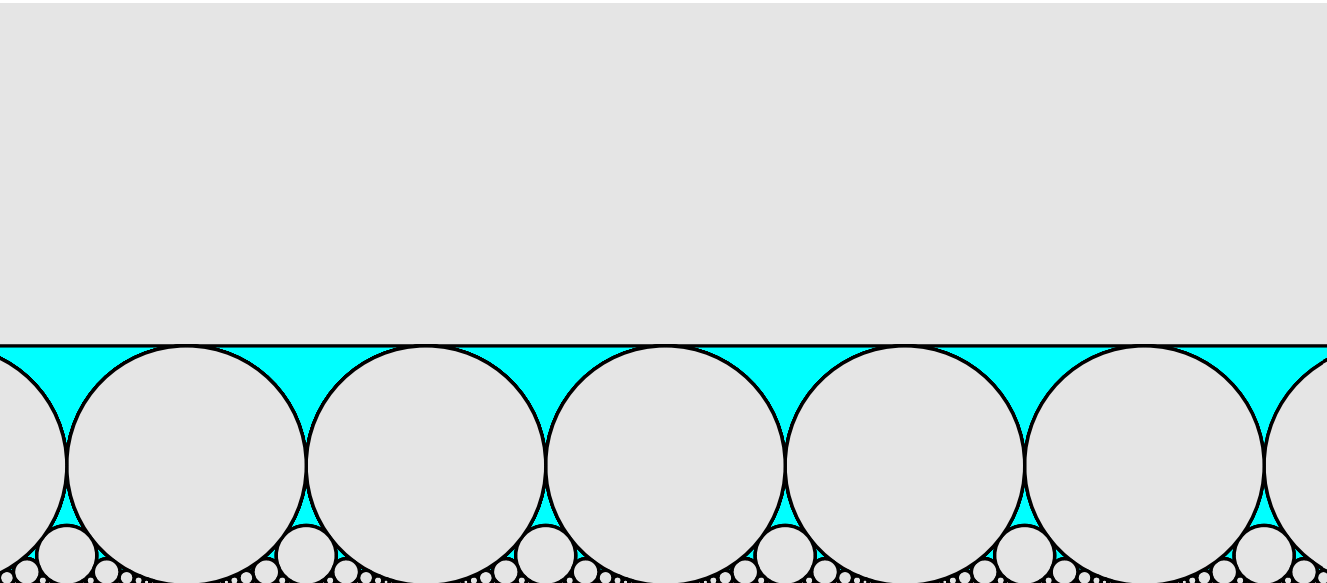
\includegraphics[width = \textwidth]{ss-locus.png}
        \caption{Semi-stable locus over $\mathbb{H}$}
    \end{figure}
\end{frame}

\begin{frame}{In higher dimensional}
We work with the lattices 

\end{frame}
\begin{frame}
    \begin{center}
        \textit{THANK YOU FOR YOUR ATTENTION.}
    \end{center}
\end{frame}
\end{document}